%-------	-------------------------------------------------------------------------------------------
%------------------------------------------------- Chapter --------------------------------------------------------
\chapter{Estado del Arte} \label{cap:estadodelarte} \label{cap:3}
%\pagenumbering{arabic} 


\section{Introducción}

Este capítulo presentará el estudio del estado del arte, partiendo de
la transformación de \textit{información de contexto} como componente de primera clase y visible en una arquitectura \ref{cap:arqdhd}, representado a través de un sistema especializado para su uso. También se suma otro componente que permite conectar un sistema externo de administración de contexto.
De esta manera, se desarrollarán las principales características de los sistemas y las estructuras que fueron utilizadas para la construcción de una propuesta de solución que determina un modelo evolutivo. 



\section{Contexto en el DHD}

En el capítulo \ref{cap:Introduccion} se referenció al contexto en
virtud de las propiedades de sistemas especializados en usar información
de contexto para brindar funcionalidades. Además, el contexto aparece como uno
de los elementos, junto a los parámetros context-aware, que forma la
pirámide de componentes de la solución propuesta (figura \ref{fig:contratosv1}).
Luego, en el capítulo \ref{cap:dhd} el contexto forma parte de la definición
conceptual del DHD como un factor a tener en cuenta para la adaptación debido a
su influencia en los \hyperref[requerimientosdhd]{RequerimientosDHD}
(\hyperref[ejemplo1]{véase ejemplos}). 

En el presente capítulo, se abordará la caracterización del contexto teniendo en cuenta la taxonomía diseñada en el DHD. Esta forma de representación posibilita describir al contexto a través de una interpretación necesaria para su tratamiento tecnológico.


\subsection {Caracterización del Contexto}

En esta tesis el contexto es considerado como  el conjunto de características, diseños y transformación de información necesarias para adaptar su funcionalidad a los usuarios. 

\subsubsection{Origen del contexto en el DHD}

En la figura \ref{fig:ontologiaContexto} se representan los orígenes de la conformación del contexto en el DHD. Las componentes grises son precisamente las diferentes fuentes donde se obtiene información de contexto. Por otro lado, las demás componentes de color blanco tienen una influencia en los procesos de su construcción. 

Existen diferentes categorías de contexto en relación a características de tipología dinámica o estática. En este sentido, los \textit{roles} y \textit{permisos} asociados a los diferentes tipos de usuarios (\textit{Miembros en formación} y \textit{Grupo Responsables}) ayudan a
caracterizar parte del perfil de un usuario. Esto permitirá ajustar determinados tipos de acciones para las diferentes herramientas (wiki, foro, videoconferencias, etc). Los servicios (ej.: agregar, borrar, etc.) que se consideran partes de las herramientas, deberán ser sensibles a la influencia del entorno teniendo en cuenta la información sintetizada que de este deviene. En este caso, en el entorno del DHD está caracterizada por información que se puede representar a través de los siguientes elementos: 


\begin{figure} 
\begin{center}
 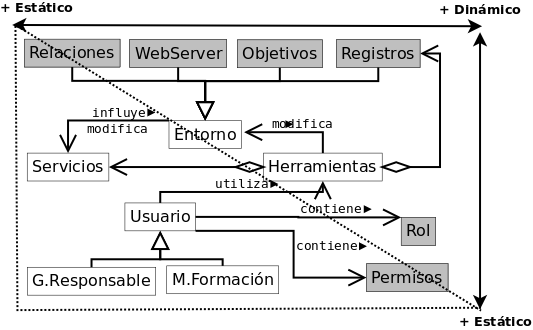
\includegraphics [width=5 in,totalheight=3 in] {Ch1/Figuras/contexto.png}
 % .: 0x0 pixel, -2147483648dpi, nanxnan cm, bb=
\caption {Fuentes del contexto del DHD}
\label{fig:ontologiaContexto}
\end{center}
\end{figure}



\begin{itemize}
 \item WebServer: información que se obtiene a partir de los \textit{logs}
del
servidor Web que permite la ejecución de las aplicación web colaborativas del
DHD. También es utilizada información de la configuración  sobre el modo
de ejecución, puertos habilitados, librerías, componentes, aplicaciones
instaladas, políticas de seguridad, tipos de sesiones, manejo y notificación
de errores, tipos de conexiones, etc.

\item Objetivos: información relacionada a los objetivos que se persiguen a
partir de ciertas configuraciones de los ambientes colaborativos del DHD. Estos
objetivos deben estar relacionados con los
\hyperref[requisitosdhd]{RequisitosDHD}
y/o \hyperref[requerimientosdhd]{RequerimientosDHD}
en los que se encuentran involucrados Stakeholder \footnote{Stakeholder es un
término inglés utilizado por primera vez por R. E. Freeman en su obra:
“Strategic Management: A Stakeholder Approach”, (Pitman, 1984) para referirse a
«quienes pueden afectar o son afectados por las actividades de una empresa».} de
forma directa o indirecta. 

\item Registros: información generada a partir de las diferentes
intervenciones de los usuarios con las herramientas que componen un espacio
colaborativo \footnote{El espacio colaborativo (Collaborative Learning) es
un conjunto de métodos de instrucción y entrenamiento apoyados con tecnología
así como estrategias para propiciar el desarrollo de habilidades mixtas
(aprendizaje y desarrollo personal y social) donde cada miembro del grupo es
responsable tanto de su aprendizaje como del de sus compañeros.}.
Habitualmente esta información aparece en forma de tablas donde se
almacena, entre otras, identificador de usuario, tiempo, la herramienta y
el servicio utilizado.

\item Relaciones: información que permite interpretar
\hyperref[interactividadDHD]{interactividades DHD} a través de la
descripción de eventos secuenciados que indican relaciones entre usuarios,
herramientas, servicios, información de contexto, sitios y otros tipo de
información tecnológica comunicacional.

\item Rol: información asociada con los usuarios de los sitios que definen
deferentes perfiles de usuarios para establecer el rol que cumplen en los procesos
colaborativos. Como ejemplo de los tipos de roles se pueden mencionar a los
``Miembros en formación``, ''Grupos Responsables``, ``Administradores'', etc
\cite{libro}.

\item Permisos: se relaciona al tipo de accesibilidad que un usuario tiene
en las herramientas de los distintos espacios colaborativos. Particularmente en
Sakai los permisos están directamente asociados con los roles. En la figura
\ref{fig:rolesSakai,fig:rolesSakai2} se muestra un ejemplo tomado de la propia
interfaz Sakai
donde se visualizan las relaciones entre un identificador de usuario y roles. 
Los permisos que permiten ejecutar las operaciones: \textit{ver}, \textit{editar}, \textit{borrar} y demás manipulación de datos asociados a las herramientas Sakai, se manejan por medio del uso de \textit{realms}
\cite{sakaimanual}. Cada \textit{realm} tiene uno a más roles para asignar a los usuarios. Los permisos son administrados a través de la herramienta \textit{Realms} \footnote{La herramienta Realms de Sakai es utilizada en la administración de permisos y roles para cada uno de los sitios.}. Se expone un ejemplo de la
estructura de \textit{permisos}, \textit{roles}, \textit{tipo} y \textit{dominios}, que se implementan en una
plataforma colaborativa Web. El anexo \ref{anexo_permisos} contiene información ampliada sobre las posibilidades de configuraciones de Sakai. A continuación se muestra un pequeño resumen para ejemplificar lo expuesto.
Véase en \cite{permisos_roles} una descripción completa. 

\begin{figure} 
\begin{center}
 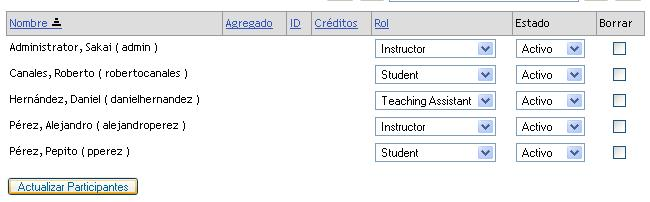
\includegraphics [width=4 in,totalheight=2 in] {Ch1/Figuras/RolesSakai.jpg}
 % .: 0x0 pixel, -2147483648dpi, nanxnan cm, bb=
\caption {Una de las interfaces para la asignaciones de roles Sakai}
\label{fig:rolesSakai}
\end{center}
\end{figure}


\begin{figure} 
\begin{center}
 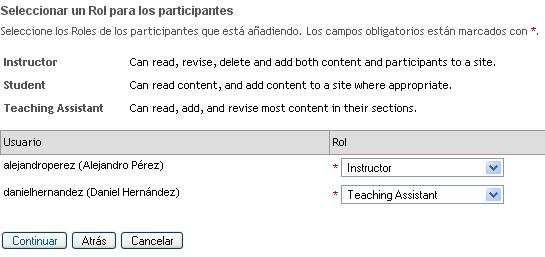
\includegraphics [width=4 in,totalheight=2 in] {Ch1/Figuras/RolesSakai2.jpg}
 % .: 0x0 pixel, -2147483648dpi, nanxnan cm, bb=
\caption {Una de las interfaces para la asignaciones de roles Sakai}
\label{fig:rolesSakai2}
\end{center}
\end{figure}



\begin{itemize}
 \item Un \textit{realm} define los permisos de ciertos objetos de la aplicación

\begin{itemize}
\item Contienen varios roles
\item Cada rol contiene determinados permisos
\item Contiene los usuarios asignados al \textit{realm} y con que rol está
asignado
\item Cada \textit{realm} indica que rol es el de mantenimiento
\item Los \textit{realms} se editan con la herramienta de ‘Edición de Realms’
\item Permite crear nuevos roles
\item Permite editar los permisos de los roles
\item Permite incluir usuarios
\end{itemize}

\begin{itemize}
 \item Los \textit{realms} se editan con la herramienta de ‘Edición de Realms’

\begin{itemize}
\item Permite crear nuevos roles
\item Permite editar los permisos de los roles
\item Permite incluir usuarios
\end{itemize}


\item Los roles por defecto de Sakai

\begin{itemize}
\item $!$site.template \rightsquigarrow  \textit{access}, \textit{maintain}

\item $!$site.template.course \rightsquigarrow \textit{Instructor},
\textit{Student}, \textit{Teaching}, \textit{Assistant}
\end{itemize}

\item Role del creador del Site

\begin{itemize}
 \item Por defecto \textit{maintain}, \textit{Instructor}
\item Está especificado por el campo mantenedor del \textit{realm}
\end{itemize}


\end{itemize}
\end{itemize}
\end{itemize}



%\subsubsection{Contexto versus información del contexto}
%\label{sec:informacionContexto}
%En la figura \ref{fig:ontologiaContexto} 


\subsubsection {Modelado del contexto} \label{sec:contextodhd}

En esta sección se muestran
algunos resultados en base al actual estado del arte que servirán como referentes
descriptivos sobre el tipo de modelo de contexto que mejor se adaptaría a las
necesidades del DHD. En este  sentido, se presenta una referencia a un metamodelo creado para un
lenguaje de desarrollo de software guiado por modelos para servicios Web
sensibles al contexto basado en UML\cite{ContextUML} 

\subsubsection{ContextoDHD: Contexto para los servicios DHD}\label{contextodhd}

Un \textit{servicioDHD}\label{serviciodhd} es un servicio con sensibilidad al
contexto que puede tener cierta flexibilidad para resolver 
\hyperref[RequerimientosDHD]{Requerimientos DHD}. Esto significa que los
servicios estarán orientados al tipo de tarea que desempeña un usuario bajo
un determinado contexto. 


Debido a la heterogeneidad de la información de contexto suministrada,
imperfecciones en la transformación de datos, información redundante, malas
interpretaciones sobres funcionalidades \hyperref[no_computable]{no
computables} y los datos cambiantes en tiempo de ejecución del entorno, es imprescindible tener una representación adecuada\cite{contextToolKit}. En particular, varios proveedores de contexto pueden estar reportando las mismas piezas (entidades y representaciones) de contexto
pero con distintas representaciones. Esto dificulta su especificación en las etapas de diseño. Por ejemplo: 

\begin{quote}
    Información inferida a partir de los datos de las interacciones anteriores de los usuarios de la aplicación. Dependiendo de las instancias de ETL, procesamiento y representación. 
\end{quote}

En los capítulos anteriores se expusieron fundamentos sobre la
importancia del contexto en el DHD y consideraciones sobre su visualización funcional a través de formas computables de representación. Por este motivo, en esta sección se presentan aspectos de
diseño sobre el estado del arte del modelado de contexto que mejor se adapta
para las representaciones en el DHD. 


En la figura \ref{fig:contextMetamodel} se muestra una adaptación del
metamodelo creado para ContextUML\cite{contextUML} que fundamenta la
creación de una sintaxis abstracta de un lenguaje considerando dos
aspectos:
\textit{modelado del contexto} y \textit{modelado de los mecanismos
de sensibilidad del contexto} (o en inglés context awareness).


\begin{figure} 
\begin{center}
 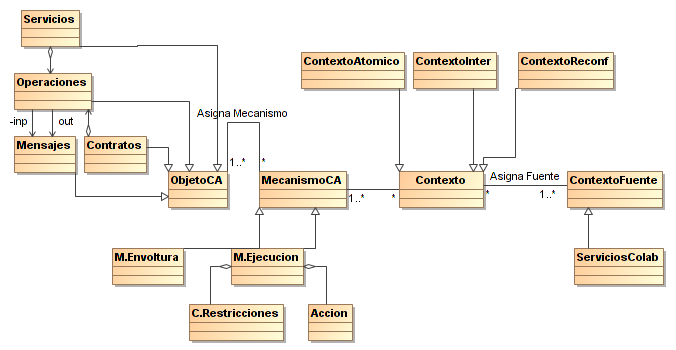
\includegraphics [width=5 in,totalheight=3 in]
{Ch1/Figuras/ContextoDHD}
 % .: 0x0 pixel, -2147483648dpi, nanxnan cm, bb=
\caption {Metamodelo del contexto para el DHD}
\label{fig:contextMetamodel}
\end{center}
\end{figure}



\textit{Contexto} es la clase que modela la información de contexto, definida anteriormente en \ref{def:contexto}, que influye en el comportamiento de los servicios de las herramientas. En nuestro diseño adaptado, el tipo de contexto está extendido en dos categorías diferentes como subtipos \textit{CotextoInter}, \textit{ContextoReconf} y \textit{ContextoAtomico}. El contexto atómico es información con el menor
nivel de abstracción posible y no comparte relación con otra porción de
contexto. Por otro lado, el contexto de las interacciones tiene que ver con
información de contexto que colabora en la descripción de las 
\hyperref[intersubjetivas]{relaciones intersubjetivas}. De la misma manera, el
contexto para la reconfiguración es una abstracción de los parámetros
\textit{context-aware} enunciados en \ref{sec:elementoscontrato}. Estos tres
subtipos agrupan a las fuentes del contexto descripto en la figura
\ref{fig:ontologiaContexto}, con lo cúal ya se cuenta con tres niveles de
caracterización del contexto para el DHD. De esta manera, se continúa con similares lineamientos utilizados en el DHD para lograr una presentación adecuada del contexto para su implementación tecnológica. 


Es claro observar que desde los servicios se encapsula (oculta) la forma de
adquirir el contexto. Así, en las implementaciones
donde intervienen servicios de herramientas se usará su misma
representación, accediendo a esta información a través de los accesos
tecnológicos de la implementación. Por ejemplo, acceso a la bases de datos,
acceso a información del servidor Web o del ambiente contenedor de los
lenguajes intervinientes (ej., Apache Tomcat \footnote{Tomcat es un servidor web
con soporte de Servlets y JSPs. Incluye el compilador Jasper, que compila JSPs
convirtiéndolas en
Servlets. El motor de Servlets de Tomcat a menudo se presenta en combinación con
el servidor web Apache.}). En otras palabras, se puede decir que el concepto de
contexto del servicio oculta la complejidad de su adquisición
bajo la perspectiva de los Sistemas Sensibles al Contexto \ref{sec:cas} (o
también mencionados como Sistemas Context-Aware).


\paragraph{Fuentes de la información de contexto}

El tipo de contexto fuente (\textit{ContextoFuente}) representa desde donde
parte los datos que construyen el contexto que luego será almacenada para su recolección, por ejemplo, en el registro de actividades. Uno de los subtipos de fuentes pueden ser los servicios colaborativos (representado por \textit{ServiciosColab}) que son utilizados en los servicios de las herramientas colaborativas (ej., Wiki, Foro, etc.). Habitualmente, esta componente están representadas en las implementaciones originales de las aplicaciones colaborativas.

Es observable que desde los servicios se encapsula (oculta) la forma de
adquirir el contexto. De esta manera, en las implementaciones
donde intervienen servicios de herramientas, se usará su misma
representación del contexto, accediendo a esta información a través de los conectores
tecnológicos implementados. Por ejemplo, acceso a las bases de datos,
acceso a información del servidor Web o del ambiente contenedor del los
lenguajes intervinientes (ej., Apache Tomcat \footnote{Tomcat es un servidor web
con soporte de servlets y JSPs. Tomcat no es un servidor de aplicaciones, como
JBoss o JOnAS. Incluye el compilador Jasper, que compila JSPs convirtiéndolas en
servlets. El motor de servlets de Tomcat a menudo se presenta en combinación con
el servidor web Apache.}). En otras palabras, se puede decir que el concepto de
contexto del servicio oculta la complejidad de de la adquisición del contexto,
bajo la perspectiva de los Sistemas Sensibles al Contexto \ref{sec:cas} (o en
inglés Context Aware System).


\paragraph{Contexto para los servicios de reconfiguración}

El subtipo representado por la clase \textit{ServicioReconf} interpreta a todos
los servicios que devienen de las reglas implementadas por los contratos, mas
precisamente, están relacionados con las acciones de estas reglas
\ref{cap:contratos}. Por otro lado, los condicionales que forman parte de las
mismas reglas se vinculan con la clase \textit{Contexto} haciendo las veces de
pre-condición; mientras que los resultados de las acciones
establecerán  post-condiciones. De esta manera se fundamenta uno de los
elementos sobre el por qué de la elección de los contratos como
pieza de software base para implementar la reconfiguración y promover la
dinámica del DHD.  



\paragraph{Modelado de la sensibilidad del contexto}

\textit{MecanismoCA} es la clase que centraliza la formalización de los
mecanismos que permiten el modelado para su implementación de las propiedades
de sensibilidad al contexto. Para este propósito se han definido dos
diferentes categorías por medio de los subtipos \textit{M.Envoltura} y
\textit{M.Ejecuciones }. Este mecanismo permitirá determinar la asociación de
la información de contexto  con objetos concretos que brindan funcionalidades
en el sistema. Estos objetos son representados por la clase \textit{ObjetosCA}.
Hay 5 subtipos de \textit{ObjetosCA}: Servicios, Operaciones, Mensajes, Partes y
Contratos. Cada servicio ofrece varias operaciones y cada operación pertenece
a un sólo servicio. Este vínculo se representa por una relación de
agregación. Cada operación tendrá un mensaje de entrada y/o uno de salida
con la posibilidad de que esos mensajes tengan metadatos (i.e.,
mensajes con parámetros). La otra posibilidad es que en vez de mensajes se
utilicen, con el mismo propósito, contratos para establecer igual tarea de
comunicación con el agregado de mayores propiedades semánticas.
Para este caso se estable una nueva relación de agregación entre
\textit{Operaciones} y \textit{Contratos}.


\subparagraph{Mecanismos de Envolturas}
El subtipo de \textit{M.Envolturas} modela los procesos automáticos de envoltura
o vinculación de la información de contexto para que pueda ser procesada por
los mecanismos de sensibilidad al contexto. Por ejemplo, en el caso que una
operación tome como parámetro un conjunto de caracteres (``string``) para
identificar un \textit{tema} de un foro, supongamos que un usuario tiene
intervenciones en dicho tema del foro con información de contexto referente a su
rol (ej., ''perteneciente al grupo responsable``). Entonces, el mecanismo
envoltura debe vincular el parámetro \textit{tema} con el \textit{rol grupo
responsable}.

Una vinculación automática de contexto (e.i., una envoltura de contexto) es
una asignación (''mapping'') entre un contexto y un objeto sensible al
contexto (ej., un parámetro de entrada de una operación de servicio). La
semántica se refiere a que un valor del objeto es reemplazado por un valor de contexto.
Cabe aclarar que el valor de un objeto sensible al contexto puede derivar varios
valores de contexto. 
 

\subparagraph{Mecanismos de Ejecución}

El subtipo \textit{M.Ejecución} modela la situación de la adaptación de
contexto
donde los servicios pueden ser ejecutados o modificados según la información
de contexto. Un contexto del mecanismo de ejecución contiene dos partes: un
conjunto de restricciones de contexto (\textit{C.Restricciones}) y un
conjunto de acciones (\textit{Acciones}), donde la semántica de esas acciones
pueden ser ejecutadas si
y sólo si se cumplen todas las restricciones impuestas para el contexto. 

Las restricciones de contexto especifican que ciertos contextos deben reunir
determinadas condiciones con el propósito de cumplir ciertas operaciones.
Formalmente, una restricción para el contexto puede estar modelada como un
predicado\cite{ContextUML} (i.e, una expresión booleana) que consiste en un
operador y dos o más operando. En los lugares donde interviene el contrato
estas expresiones podrán ser representadas como parte de los condicionales
de las reglas. En el caso que esto no ocurra, \textit{M.Ejecución} será el
encargado de implementar las restricciones. Un ejemplo de estas expresiones
puede ser: 

\begin{verse}

\begin{verbatim}
tema_foro='\%DHD\%' and id_foro=1233
\end{verbatim}               

\end{verse} 


para indicar que el operador se ejecutará si se está en un Foro, identificado con el número “1233”, donde el tema tenga el string “DHD”. Esta forma de interpretación posibilita además poner en la misma expresión de acciones para el caso que no se cumpla la condición.

Existe un lenguaje para ContextUML\cite{ContextUML} que puede ser usado para
este mismo modelo de contexto en la programación de acciones desde
el propio mecanismo que implementa la sensibilidad al contexto. En esta tesis,
es de interés utilizar solamente el modelo de contexto y todas las acciones de
adaptabilidad serán mediadas por la componente contrato. 




\section{Sistemas Sensibles al Contexto} \label{sec:cas}


En esta sección se toma el antecedente de la representación y
formas de utilización del contexto, información de contexto, mecanismos de
manipulación y las fuentes de recolección en el DHD. El propósito es
interpretar la posibilidad de agregar a un sistema
colaborativo Web (original) las propiedades de sensibilidad del
contexto creadas para el DHD (ContextoDHD).

Podemos entender a un sistema colaborativo sensible al
\hyperref[contextodhd]{contextoDHD} cómo una
aplicación provista de mecanismos que permiten una mejor adaptación de los
servicios a partir del contexto de los usuarios y del entorno. En ambientes
colaborativos para educación, los servicios forman parte de las funcionalidades
observables, desde las perspectivas de los usuarios (ej.: alumno, docente, etc.),
que proveen las herramientas de la Aplicación (ej., wiki, foros, mensajería,
glosario, recursos, etc.). Los elementos que componen la caracterización del
contexto deben pertenecer a un dominio bien definido, manteniendo ciertos
niveles de concordancia con los mecanismos encargados de manipularlos y la toma
de decisiones basándonos en ellos.

A través de un simple diagrama, es posible observar algunas de las características
fundamentales que determinan un sistema colaborativo sensible al contexto,
donde se
encuentran remarcadas aquellas particularidades (tecnológicas y
conceptuales) que se vinculan con la perspectiva del DHD. En la figura
\ref{fig:evolucion}, describimos desde una arquitectura básica y genérica, tres
tipos de niveles, cada uno agrega nuevos rasgos y comportamientos que
condicionan los servicios del dispositivo hipermedial hacia un nuevo modelo.

\begin{figure}
\begin{center}
 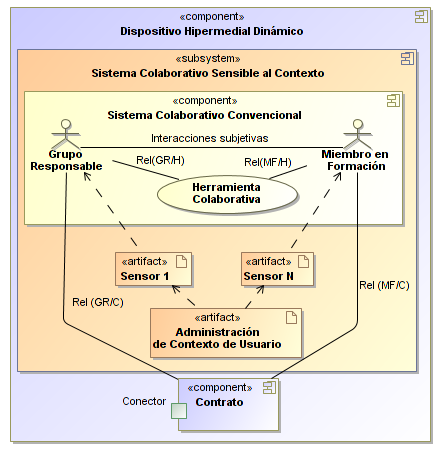
\includegraphics[width=3.5 in,totalheight=3.5in] {Ch1/MEvolutivo.png}
 % .: 0x0 pixel, 0dpi, 0.00x0.00 cm, bb=
\caption{Arquitectura propuesta evolutiva.}\label{fig:evolucion}
\end{center}
\end{figure}

La figura está dividida en tres bloques fundamentales, en el primero (Sistema
Colaborativos Web Convencional) se describen los principales componentes y
relaciones; fundamentalmente un alumno puede interactuar con las herramientas y
servicios del sistema y comunicarse con un docente o con sus pares.


El segundo bloque de la figura (Sistema Colaborativo Sensible al
Contexto) contiene el
agregado de dos componentes esenciales, sensores y un administrador de contexto.
Los
sensores capturan información del usuario y del entorno, son partes
fundamentales para
la recolección de información; si los sensores juegan un papel secundario, los
podemos
enmarcar bajo el concepto de artefactos virtuales. El segundo componente hace
referencia a la administración del contexto, donde se destacan las siguientes
funcionalidades: recolección, abstracción, interpretación, comunicación y
almacenamiento. Para la implementación de comportamientos context-aware los
diseños de software deben completarse con diferentes modelos, para el caso de
los
denominados sistemas e-learning, las soluciones se focalizan en la tecnología de
comunicación e información que utilizan los usuarios. MatchBase (Gross et al.,
2006)
es un proyecto de referencia en cuanto al uso de estos tipos de diseño y
tecnología,
conformando una herramienta para el desarrollo de comunicaciones contex-aware.
Fue
trasladado como experiencia a proyectos de investigación de sistemas e-learning
context-aware (Schmidt, 2005). Pensar en aplicaciones para educación e
investigación sensibles al contexto dentro del marco teórico context-awareness
conforma un nuevo paradigma, donde las relaciones (rotuladas con “Rel
(fuente/destino)” en la figura) cobran un mayor protagonismo en la concepción de
los marcos conceptuales propuestos como soluciones a nuevos requerimientos
académicos para el contexto físico-virtual.


Perspectivas como la del DHD, también centran los requerimientos sobre
las relaciones y comunicaciones entre los principales componentes del
dispositivo,
focalizados en las relaciones entre los actores (Recursos Humanos en formación,
grupos
responsables) y los servicios brindados por las herramientas anteriormente
mencionadas, a las que se les integra el potencial de comunicación hipermedial
como
por ejemplo, video conferencias, edición en variados formatos, etc.

Retomando la evolución de los sistemas colaborativos referida a la adaptación de
modelos
para requerimientos educativos complejos, el último bloque de la figura
(Dispositivos
hipermediales sensibles al ContextoDHD Dinámico) representa un modo de
interpretación de una
nueva configuración de la arquitectura de un sistema, debido a la interposición
de la
componente contratos (referenciada con el dibujo característico para componentes
de
software en UML). Al agregar este nuevo elemento que permite una mejor
articulación
de las relaciones, resulta una nueva teoría que proporciona conceptualmente un
marco
innovador para las prácticas de diseño, desarrollo, uso de dispositivos y
aplicaciones en dicho campo.


El contrato debe ser visto como una alternativa de abstracción de las relaciones
mencionadas anteriormente, determina un nuevo tipo de relación que mantiene las
características de los anteriores bloques de la figura y además, reduce la
complejidad de
los modelos de los SSC en la adaptación de los servicios que interfieren
en
relacionamientos entre usuarios y comunicacionales. Los contratos se nutren con
información del contexto por medio de sus parámetros; no intervienen en la
recolección,
ni en la abstracción, ni en la distribución del contexto y en principio pueden
ser
adaptados a cualquier modelo de sensibilidad al contexto similar, bajo la
perspectiva propuesta por Dey. et. al (2001).


A continuación, se analizan las principales características de los
SSC.
Como observamos en la figura anterior, el bloque intermedio se configura como
articulador entre los sistemas colaborativo tradicionales y las
nuevas posibilidades
tecnológicas que permiten la concreción más efectiva del Dispositivo
Hipermedial
Dinámico agregando la componente Contrato.

Esta propuesta evolutiva y la forma de representación del contexto mantiene
los principios que definen la teoría de los SCC.

El contexto puede definirse de manera general como:

\begin{quote}
Cualquier información que puede usarse para caracterizar la situación de
una entidad. Donde una entidad es una persona, lugar u objeto que es
considerado relevante para la interacción entre un usuario y una
aplicación, incluyendo al usuario mismo y la aplicación.
\begin{flushright}(Dey y Abowd, 2000)\end{flushright}
\end{quote}  


Las aplicaciones sensibles al contexto se definen  como:


\begin{quote}
Aquellas que usan el contexto para proveer información y/o servicios
relevantes al usuario, donde la relevancia depende de la tarea del usuario.
\begin{flushright}(Dey y Abowd, 2000)\end{flushright}
\end{quote}

Según un análisis realizado por Brown et al., (2000), entre las aplicaciones sensibles al contexto, la recuperación de información juega un papel central, y tales aplicaciones parecen confirmarse como la prospectiva que requiere el cómputo consiente (sensible) del contexto. A continuación se enuncian conceptos tomados de autores en cuyos trabajos utilizan la información de contexto con los principios anteriormente mencionados.


\subsection {Propuestas para la Identificación del Contexto} 

Algunos trabajos se han enfocado sobre cómo identificar el contexto efectivamente y cómo obtener una representación del mismo que pueda ser utilizada para incorporarlo a la búsqueda de información relevante para el usuario.

Budzik y Hammond, (2000) clasifican los esfuerzos llevados a cabo para esta tarea en cuatro categorías:

\begin{itemize}
\item \textbf{Retroalimentación sobre la relevancia de los resultados}: Trata
de determinar el contexto obteniendo cierta retroalimentación por parte del
usuario respecto al nivel
de relevancia de los resultados que pueda tener una consulta (Salton y
Buckley, 1990).


\item \textbf{Perfiles de usuario}: en este caso los intereses del usuario se
integran para formar un
perfil que es efectivo a lo largo de varias consultas, un ejemplo de este
enfoque es
Letizia (Lieberman, 1995).

\item \textbf{Eliminación de ambigüedad en el sentido de las palabras}: Algunos
sistemas tratan
de eliminar posibles ambigüedades pidiendo al usuario que lo haga explícitamente
(Cheng y Wilensky, 1997), mientras que otros, lo hacen implícitamente usando la
popularidad de los términos según la estructura interna de los documentos de
hipertexto (Bradshaw y Hammond, 1999).

\item \textbf{Enfoques de ingeniería del conocimiento}: intentan crear un modelo
de
comportamiento del usuario mientras estos se encuentran interactuando con una
aplicación.
\end{itemize}

A su vez, Lawrence (2000) propone cinco tipos de estrategias para incluir el
contexto en
las búsquedas:

\begin{itemize}

\item \textbf{Agregar información de contexto en forma explicita}: se presentan
al usuario
mecanismos para que éste especifique el contexto en el cual desea realizar su
búsqueda. Tal es el caso del proyecto Inquirus 2 (Glover et al., 2000).

\item \textbf{Inferir la información de contexto automáticamente}: los sistemas
tratan de obtener
dicha información de contexto sin la intervención conciente del usuario,
usualmente
monitoreando las actividades y aplicaciones de éste. El proyecto Watson (Budzik
y
Hammond, 2000) se inscribe en esta categoría. Siguiendo este mismo enfoque hay
sistemas que recomiendan enlaces a sitios Web dinámicamente mientras el usuario
realiza sus tareas, algunos ejemplos de este tipo de sistemas son: The
Remembrance
Agent (Rhodes, 2000), SurfLen (Fu et al., 2000), Margin Notes (Rhodes, 2000), y
Fab (Balabanovic, 1997).

\item \textbf{Búsquedas personalizadas}: este concepto implica que una máquina
de búsqueda
conozca todas las búsquedas anteriores del usuario y que use esa información
para
personalizar los resultados de búsquedas futuras. Con el buscador Northern Light
el
usuario recibe notificaciones sobre nuevas páginas que concuerden con ciertas
expresiones de búsqueda.

\item \textbf{“Adivinar” lo que el usuario quiere}: este enfoque consiste en
examinar la expresión
de búsqueda del usuario y cuando se encuentran ciertos términos predefinidos el
buscador arroja en los resultados ciertas páginas asociadas a tales términos.
Google
(www.google.com) percibe una cadena de caracteres que tiene el formato de una
dirección, arroja resultados con enlaces a mapas de esa zona. Otros ejemplos son
(www.excite.com) y (www.lycos.com).

\item \textbf{Restringir el contexto de las máquinas de búsqueda}: otra manera
de delimitar el
contexto es restringir el dominio de la misma máquina de búsqueda. 

\end{itemize}


Actualmente, disponemos de gran diversidad de buscadores especializados, algunos
ejemplos son:
CiteSeer (Lawrence et al., 1999) y Deadliner (Kruger et al., 2000). También existen meta buscadores que implementan algún mecanismo para derivar el contexto del usuario y luego usan esa información para realizar consultas sobre alguno de estos buscadores especializados. Tal es el caso de Inquirus 2 (Glover et al., 2000).

Sobre los enfoques para “Derivar el contexto pasado y futuro”, Brown y Jones (2002), proponen explotar la característica del contexto que lo hace cambiar constantemente, pero en cierta medida de manera predecible.

Al analizar cómo es el proceso de cambio y llevar un registro del mismo, podemos crear lo que dichos autores llaman: “Diario de Contexto”, guardando los estados de las variables de contexto medidas por sensores, ya que a través de esta información se puede predecir un contexto de interés a futuro. También proponen un "Context-aware Caching" (depósito de documentos) en el cual, se recupera la información, haciéndolo con un contexto en donde los campos (o variables) son rangos estimados de valores que puede tomar cada campo en un futuro cercano, utilizando los documentos resultantes para formar un depósito temporal desde el cual se pueden realizar mas rápidamente recuperaciones posteriores mientras el contexto del usuario no cambie considerablemente.

\subsection {Visiones en la perspectiva histórica}
 
Es interesante considerar, en el marco de esta tesis, algunos de los antecedentes más relevantes a nivel histórico del paradigma que subyace en los sistemas sensibles al contexto, citaremos a continuación estacados referentes:

\paragraph {Vannevar Bush's Memex (1945)}

Propone, antes del desarrollo del computador, un aparato denominado Memex que, como suplemento de nuestra memoria, facilitaría el acceso y la relación de la información acumulada. La clave de este dispositivo, es que funcionaría imitando los procesos de asociación de la mente humana. Reconocido el límite que impone el artificio, se plantea igualmente un cambio fundamental: la selección debe ser por asociación y no por la ubicación mecánica de temas en un índice alfabético.

En el Memex se podrían guardar archivos, libros y textos para ser consultados con rapidez y flexibilidad, sería posible agregar comentarios y notas marginales.

Quien consultara, construiría senderos de lectura de acuerdo a su interés, seleccionando y enlazando los artículos a través del laberinto de materiales disponibles, y podría modificar esta configuración cuando lo deseara. Bush concretiza a nivel de objeto tecnológico la recuperación y escritura de la información en formato hipertextual.

Edward Thorp: “The invention of the first wearable computer” (1960) La primera computadora “wearable” (que se puede llevar puesta en el cuerpo) fue concebida en 1955 por Edgard Thorop para predecir el comportamiento de la ruleta, culminando en un trabajo conjunto en el M.I.T. con Claude Shannon en 1960-61. El dispositivo era similar al tamaño de un paquete de cigarrillos y permitía aumentar hasta un 44\% las chance de ganar, si bien se probó el objetivo planteado, luego ocurrieron pequeñas fallas en el hardware que impidieron continuar con el uso de este dispositivo. Este método y la existencia de la computadora no fueron publicados hasta el año
1966.


\paragraph {Alan Kay's Dynabook (circa 1977)} 

La Dynabook es un dispositivo portátil, con red inalámbrica y pantalla plana, entre otras cosas. Este dispositivo se concibe como extensión de las posibilidades de la mente-cuerpo y lugar donde un usuario concentra toda la información que consume y que genera. Guiados por esta visión, un grupo de referentes de la informática (Alan Kay, Dan Ingalls, Adele Goldberg, etc.) fueron responsables de los desarrollos de mayor impacto relacionados con las computadoras personales. Una lista, no completa, de los aportes de este proyecto son: “El concepto de la Computadora Personal”, “El paradigma de objetos”, “Smalltalk”, “Interfaces de usuario gráficas”, “Uso del Mouse”, “Drag& drop”, “Menúes desplegables”.

Las ideas de la Dynabook siguen vigentes en el Squeak y su filosofía en grupos como SqueakLand. Los eToys y los Ensayos Activos son subyacentes a las ideas del meta-medio.


\paragraph {Mark Weiser; “The Computer for the 21st Century (1991)}  

La computación ubicua como paradigma de interacción fue introducida por Mark Weiser en 1991 después de sus trabajos en los laboratorios de Xerox PARC en Palo Alto (Weiser, 1991). La computación ubicua pretende ampliar la capacidad computacional a todo el entorno mediante la distribución de pequeños y muy diversos
dispositivos que presentan ciertas características interactivas, todos ellos conectados a
servidores de mayor potencia.

El diseño y situación de estos dispositivos debe estudiarse rigurosamente, según la tarea que realizan. De este modo, la responsabilidad computacional se desplaza diluyéndose en el entorno (transparencia del objeto computacional), intentando suscitar la idea de omnipresencia (Norman, 1998). La solución propuesta por Weiser (1991-1998) fue disponer de redes inalámbricas para computadoras con la finalidad de intercambiar
información entre ellas y configurar un dispositivo de interacción. En los ambientes ubicuos hay tres tipos de computadoras: “marcas”, “tabletas” y “pizarras”.

En el Centro de Investigación de Xerox de Palo Alto, diseñaron estas computadoras, (Ubicom) y Weiser en 1998, sostuvo que su propuesta podría tener mayor aceptación en los campus universitarios. En 1999, distintos equipos de investigación adoptan internacionalmente con fines educativos este nuevo paradigma para el aula.
Soloway et. al (1999) expuso el beneficio que esto significaría para el aprendizaje por descubrimiento, mediante la realización de experiencias que surgen a partir de los principios del paradigma de computación ubicua, al considerar estos dispositivos como controles remotos de una pizarra de grupo. El mencionado investigador, proponen
diseñar dispositivos y periféricos que sirvan para captura de datos en el entorno real mediante la utilización de dispositivos handheld. Posteriormente, estos datos serían enviados a un servidor que los presentará para su discusión grupal.


\paragraph {Bill Schillit: “Context-Aware Computing Applications” (1994)}
  
Schilit define computación context-aware por medio de la caracterización de aplicaciones context-aware de la siguiente manera:

Selección próxima: una técnica de interface de usuario donde el objeto más próximo es señalado o facilitado para su mejor selección.

\begin{itemize}
 \item Reconfiguración automática de contexto: es el proceso por el cual se agrega un nuevo componente, se quita un componente existente, o se altera la conectividad entre dos componentes ante un eventual cambio en los elementos que componen el contexto.

\item
Información de Contexto y comandos: los cuales pueden producir diferentes resultados de acuerdo al contexto que donde se utilizan.

\item Lanzamiento de Acciones ante cambios de Contexto: son simples reglas tipo IFTHEN utilizadas para especificar cómo se debe comportar el sistema context-aware.
\end{itemize}



\paragraph {Don Norman: “The invisible Computer” (1998)}

A partir de los años ’80, con la difusión masiva de las interfaces user-friendly, se consolida entre muchos proyectistas e investigadores una concepción que privilegia una lectura sobre la interacción hombre-computadora en términos instrumentales y que tiende a hacer "desaparecer" la interfaz. Don Norman, propone que los mejores programas informáticos "son aquellos donde la computadora 'desaparece’ y se puede trabajar sin tener en cuenta a la máquina." (1989:231). Esta aparente "invisibilidad de los procesos de interacción" es una consecuencia directa de la aplicación de la metáfora mcluhaniana sobre la extensión de las interfaces digitales como prótesis de nuestro
cuerpo. Esta perspectiva, propone que la mejor interfaz es aquella que desaparece durante el uso. Según Anceschi las interfaces deberán ser lo más transparente posible, o sea, deberían tener la menor consistencia (perceptiva) posible" (1993:19). GuiBonsiepe, sostiene que "el usuario ha aprendido el uso de un programa cuando éste se
vuelve tan transparente que ya no tiene necesidad de 'pensar’, o sea cuando el programa desaparece y el usuario puede ocuparse de la ejecución de la tarea que se propone realizar..." (1993b:52). De Kerckhove, afirma que antes de alcanzar el nivel de saturación una tecnología debe atravesar dos fases: en la primera el dispositivo
resulta muy evidente, en la segunda se interioriza "hasta volverse invisible" (De Kerckhove, D.:1999, 123).

\section{Componentes bases para los Sistemas Sensibles al Contexto}\label{requisitoDHD}
  
En esta sección, expondremos los diferentes tipos de componentes para capturar contexto que integran un Modelo para la Sensibilizarlo al Contexto (MSC). Particularmente, mencionaremos dos tipos de moles emblemático con diferentes enfoques.

\subsection{Context Toolkit}

En primer lugar, se analiza un modelo tradición fundador expuesto en la tesis doctoral de Dey (2003)\cite{dey}. La siguiente tabla muestra una clasificación de arquitecturas en las que se resaltan las principales características:

\begin{quotation} 

\begin{itemize}
\item Acceso directo a Sensores:
	    \begin{itemize}
	       \item No extensible
	       \item Componentes altamente acopladas
	    \end{itemize}

\item Basado en Middleware: 	   
	      \begin{itemize}
	       \item Permite la ocultación de detalles de censado de bajo nivel.
	       \item Extensible.
	       \item Permite el acceso de múltiples clientes a los datos de
forma remota.
	       \item Libera a los clientes de recursos que demandan
	      \end{itemize}

\item Servidor de Contexto:operaciones intensivas.
	    \begin{itemize}
	       \item Debe considerar el uso de protocolos apropiados, rendimiento
de la red, calidad de lo parámetros de los servicios.
	    \end{itemize}

\item Widgets:
	  \begin{itemize}
	  \item Encapsulamiento.
	  \item Intercambiable.
	  \item Controlado a través de un manejador de widget.
	  \item En el caso de que las componentes estén acopladas, incrementan la
	  eficiencia, al costo de perder robustez ante fallas de componentes.
	  
	  \end{itemize}
\item Networked services:(modelo orientado a objeto) 
	\begin{itemize}
	\item Similar a la arquitectura Servidor de Contexto.
	\item No tiene la eficiencia de la arquitectura widget debido a la
    complejidad
	de las componentes bases de red, pero provee robustez.
	\end{itemize}

\item Blackboard model: (modelo basado en datos) 	
	\begin{itemize}
	\item  Procesos pos-mensajes para compartir medios, pizarrón.
	\item Simplicidad en el agregado de nuevos recursos de contexto.
	\item Fácil configuración.
	\item Un servicio centralizado.
	\item Carece de eficiencia en la comunicación (son necesarios dos puntos
	de conexión por comunicación). 
	\end{itemize}

\end{itemize}                                
\end{quotation} 


Llegado a este punto, introduciremos una definición de la componente
principal del modelo: el Widget.


Este componente, deriva del homónimo elementos GUI, un Widgets es un componente de software que brinda una interface pública para algún tipo determinado de sensores (hardware) (Dey and Abowd, 2000, 2001). Los Widgets ocultan detalles de censado de bajo nivel y al mismo tiempo son componentes con alto grado de reusabilidad, facilitando el desarrollo de aplicaciones. El encapsulamiento en los Widgets permite intercambiarlos entre aquellos que proveen el mismo tipo de datos (ejemplo: intercambiar un Widget de radiofrecuencia por un Widget de una cámara filmadora donde ambos recolectan datos de locación de individuos).


Usualmente los Widgets son controlados por alguna clase de administrador de widget.
En el caso de que las componentes sean acopladas incrementan la eficiencia, al costo de perder robustez ante fallas de componentes. Se identifican cincos categorías de componentes que implementan distintas funciones:

\begin{itemize}

\item 
\textbf{Context Widgets}: se encarga de la adquisición de información de
contexto.

\item
\textbf{Intérpretes}: cumplen la función de transformar y aumentar el grado de
abstracción de la información de contexto; deben combinar varias piezas de
contexto para producir información procesada de alto nivel.

\item
\textbf{Aggregator}: es un componente que junta información de contexto de una
entidad para facilitar su acceso a las aplicaciones.

\item
\textbf{Services}: brindan servicios en un determinado ambiente adaptando su
funcionalidad al tipo de información de contexto adquirida.

\item
\textbf{Discoveres}: permite que las aplicaciones (y otras entidades) optimicen
su desempeño pudiendo determinar la característica del entorno (tipo de
restricciones y dominio de aplicación). Entre estos componentes se pueden
establecer un número limitado de relaciones.

\end{itemize} 

Widgets es consultada, o bien, notificada ante eventuales cambios en los clientes. Los
clientes pueden ser aplicaciones, Aggregators u otros Widgets. A su vez Aggregators actúa como un puente entre Widgets y aplicaciones. Un Interpreters puede ser solicitado en un determinado estado por un Widget, Aggregator o aplicaciones. Los Services son lanzados por las aplicaciones (también otros componentes pueden hacer uso de los servicios). Discoveres se comunica con todos los componentes, adquiere desde los Widget, Interpreters y Aggregators, y provee información a las aplicaciones por medio de notificaciones y consultas.

La figura \ref{fig:deytoolkit} expone una posible configuración con dos dispositivos de censado, dos Widgets, un Aggregator, dos Interpreters, un servicio, un Discoverer y dos aplicaciones.

\begin{figure}
\begin{center}
 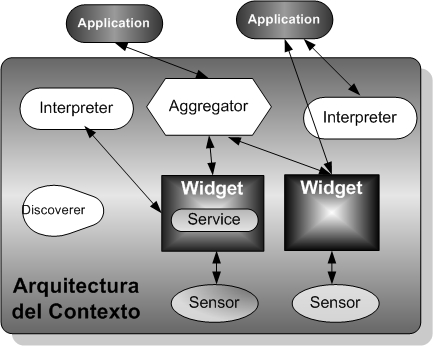
\includegraphics [width=5 in,totalheight=4 in] {Ch1/f2.jpg}
 % .: 0x0 pixel, -2147483648dpi, nanxnan cm, bb=
\caption {Una configuración de las componentes del Context Toolkit.}
\label{fig:deytoolkit}
\end{center}
\end{figure}

En el instante en que algún componente contexto se encuentre disponible,
registra sus capacidades en un \textit{Discoverer}. Esto permite que los \textit{Aggregators}
encuentren \textit{Widgets} e\textit{Interpreters} y a las aplicaciones encontrar \textit{Aggregators}, \textit{Widget} e \textit{Interpreters}. Un sensor provee datos para un \textit{Context Widget}, en cuál se encarga de almacenar el contexto, a su vez, puede llamar a un \textit{Interpreter} para obtener un mayor nivel de abstracción de los datos y luego pone el contexto a disposición, para poder ser accedido,  por otros componentes y aplicaciones. Un \textit{Aggregator} recolecta información de contexto de las entidades, representadas por los \textit{Widgets}. Finalmente, las aplicaciones pueden consultar o suscribirse a los \textit{Agreegators} (o directamente con los \textit{Widgets}, si se quiere) y llamar a \textit{Interpreters} (si el deseado nivel de abstracción no se encuentra disponible desde los
\textit{Widgets} y \textit{Aggregators}).

Estos componentes se ejecutan independientemente de las aplicaciones, asegurando una continua adquisición de información de contexto y el uso de múltiples aplicaciones.

Además, todos los componentes y aplicaciones se comunican entre ellos automáticamente usando protocolos y lenguajes conocidos. Esto da lugar a que los programadores que implementaron un particular componente o aplicación puedan comunicarse con otro componente sin tener conocimiento de los mecanismos usados para lograr la interacción.


\subsection{Proyecto UWA}

UWA ha nacido de la colaboración entre diferentes grupos de trabajo, por lo que resulta realmente una agrupación de propuestas y técnicas. UWA incluye una original propuesta de aplicar la notación UML para modelar elementos de multimedia que a su vez es heredado de otra propuesta llamada HDM (Hypermedia Design Model)\cite{HDM11}. Sin embargo, la metodología de desarrollo W2000 ha sido incluida en UWA sólo en la fase de diseño hipermedia, siendo ambas propuestas diferentes en la fase de definición de requisitos. Por esta razón han sido incluidos en este proyecto en forma separada. El proceso de captura de requisitos en UWA\cite{UWA32} comienza definiendo los diferentes roles de usuario que pueden interactuar con el sistema, los objetivos globales del sistema y la relación entre estos. El proceso continúa haciendo un refinamiento de esos objetivos globales, concretándolos en sub-objetivos. Estos sub-objetivos son estudiados y refinados para detectar conflictos entre ellos. De esta forma, se concretizan aún más dividiéndolos en requisitos. Los
requisitos son clasificados en varios tipos: de \textit{contenido}, de \textit{estructura de contenido}, de \textit{acceso}, de \textit{navegación}, de \textit{presentación}, de \textit{operaciones de usuario} y de
\textit{operaciones del sistema}. 

De esta forma, los requisitos se van refinando hasta que solo pertenezcan a uno de estos grupos. Y finalmente los requerimientos son asignados a artefactos de diseño o a reglas de customización.
Para definir los objetivos, UWA propone una notación propia, basada en una plantilla. La definición de los actores y la relación con los objetivos se hace usando un diagrama basado en casos de uso. Por último,
para definir y refinar los sub-objetivos y los requisitos, utilizan una notación gráfica propia que denominan grafo de refinamiento de objetivos, el refinamiento de este grafo permite ir representando la relación entre los requisitos y hacer un seguimiento para validar la consecución de los objetivos del sistema. Una vez que los requisitos son detectados, hacen uso de XML para definirlos de una manera formal.


\begin{quote}
''An ubiquitous web application is a Web application that suffers from the anytime/anywhere/anymedia syndrome. This means that an ubiquitous web application should be designed from the start taking into account
not only its hypermedia nature, but also the fact that it must run “as is” on a variety of platforms, including mobile phones, Personal Digital Assistants (PDAs), full-fledged desktop computers, and so on. This
implies that an ubiquitous web application must take into account the different capabilities of devices comprising display size, local storage size, method of input, network capacity, etc. New opportunities are
offered in terms of location-based, time-based, and personalised services taking into account the needs and preferences of particular users. Consequently, an ubiquitous web application must be, on the one
hand, context-aware i.e., aware of the environment it is running in, and on the other hand it must support personalisation From: Ubiquitous Web Application Development- A Framework for understanding``

\begin{flushright}
\textit{A. Finkelstein et al 2002}
\end{flushright}
\end{quote} 


Se comienza con la descripción conceptual del framework propuesto en el proyecto UWA para el desarrollo de aplicaciones web ubicuas basada en el enfoque de la teoría reflexión (\textit{reflection})



\begin{figure}[t]
\begin{center}
 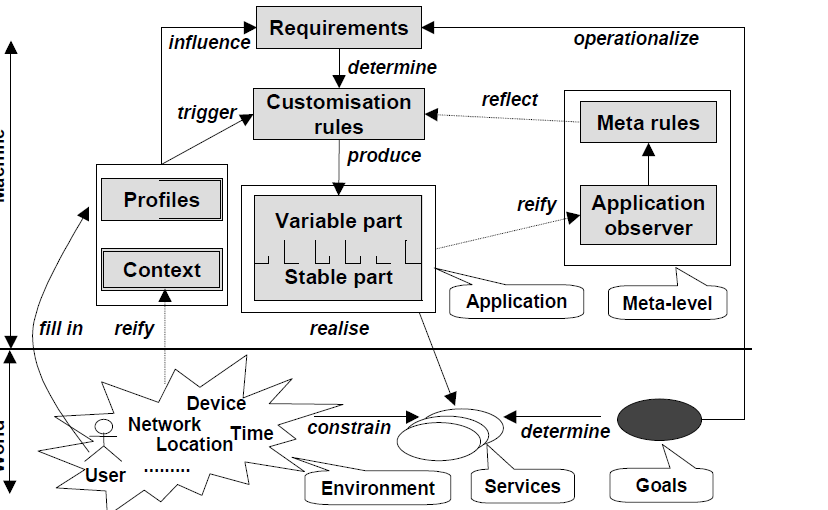
\includegraphics[width=5 in,totalheight=4 in] {Ch1/Figuras/UWAFramework2.png}
 % UWAFramework2.png: 828x510 pixel, 96dpi, 21.90x13.49 cm, bb=0 0 621 382
\caption{Diseño conceptual del Framework UWA}\label{fig:uwaFramework}
\end{center}
\end{figure}



\paragraph{Goal:}

Goal es un objetivo que el sistema debe alcanzar por medio de la cooperación entre agentes (usuarios y componentes  software) propiamente dicho y dentro de un entorno. Desde la perspectiva UWA los objetivos son \textit{inmutables} i.e., no cambia ante cuando se modifica el entorno. Representa el último objetivo que el servicio está destinado a lograr. Un cambio en los objetivos significaría cambiar el servicio mismo. A lo largo de las líneas de \cite{UWA5}, donde un “goal” no es alcanzado por una “acción directa” de uno a más agentes. De otro modo, un “goal” se convierte en un objetivo un tanto
abstracto de largo plazo.

En la Figura \ref{fig:uwaFramework}, los objetivos son de color gris, lo que significa que ellos son la única parte del marco que no tiene la intención de cambiar en tiempo de ejecución. Más exactamente, las metas pueden (y deben) tener una imagen en tiempo de ejecución (ya que su puesta en marcha en los requisitos de forma dinámica puede cambiar), pero no se pueden modificar directamente.

\paragraph{Service:}

El servicio se puede definir como algo que proporciona valor añadido a uno o más actores. Un servicio es distinto de
una aplicación, ya que es un concepto mucho más general, que podría ser proporcionada, por ejemplo, por medios distintos de
computadoras. Por ejemplo, si uno de los objetivos es maximizar la usabilidad del sistema, un servicio puede ser el de proporcionar a los usuarios con los dispositivos de entrada-salida. Este es un ejemplo de diseño centrado en el
usuario, mediante el cual el sistema es sólo un medio para cumplimiento de las metas de usuario, y no un objetivo en sí mismo. Por lo tanto, los servicios deben pertenecer en el mundo, no en la máquina.


\paragraph{Environment}

Por "Environment" se refiere al entorno en que la máquina operar. Teniendo en cuenta el medio ambiente es crucial porque influye significativamente en el comportamiento de la máquina.

El entorno cuenta con propiedades para describir una faceta diferente del medio ambiente. Consideremos el ejemplo de un
servicio relacionado operaciones de compra electrónica realizado por un usuario a través teléfono celular (m-commerce). En este caso, el medio ambiente abarca cosas tales como ancho de banda, la ubicación absoluto y relativo, la disponibilidad del
servicio, las características del dispositivo, y muchos temas más.

Se debe tener en cuenta que el sistema no tiene control alguno sobre el medio ambiente, lo que significa que la máquina debe adaptarse al medio ambiente, no al revés. Si el ancho de banda es limitado, la conexión es irregular, la pantalla del dispositivo es pequeña, esto es algo que no puede ser modificado directamente por el software. Por lo tanto, el trabajo del ingeniero de software se resume en enfrentar los desafíos del entorno y trabajar hacia la meta, utilizando el entorno tal como es y describiéndolo de la mejor manera posible, aunque no podemos cambiarlo.


\paragraph{Context}

Contexto se define como la resignificación del medio ambiente en términos de sus propiedades. En la figura, desde el contexto no salen flechas hacia el entorno medio ambienta ya que UWA lo interpreta como no modificable. A su vez, el contexto permite efectuar una descripción del medio ambiente. La mayoría de las descripciones importantes deben ser dinámicamente 
actualizablesen función del cambio posible del medio ambiente. 

Es importante destacar que el contexto es una parte fundamental de la máquina, ya que representa el entorno que pertenece al mundo real y que existe dentro del sistema. De hecho, el contexto es la única parte del sistema que es independiente de la aplicación que se construye, ya que describe las propiedades del entorno adecuado para cualquier aplicación en particular. Esto se muestra en la figura \ref{fig:uwaFramework} mediante un doble contorno alrededor de la caja de contexto.


\paragraph{Profiles}

A diferencia del contexto, el perfil representa información explícita. Un ejemplo es el uso de perfil para la personalización de usuarios. El perfil puede ser dependiente o independiente de la aplicación.


\paragraph{Requirements}

Los Requerimientos representan una de las posibles formas de lograr una meta. Un requerimiento personaliza un objetivo, ya
que representa en una forma más concreta los objetivos a corto plazo que son directamente alcanzables a través de las acciones realizadas por uno o más agentes. Los requisitos pueden cambiar durante la ejecución del sistema. El entorno pude sufrir un alto grado de cambio invalidando los objetivos iniciales. Entonces, cambios en el contexto puede generar la necesidad de cambios en los requerimientos.

En términos informal, se puede decir que los requisitos son un ''trade-off'' entre los  objetivos y la realidad actual. Por ejemplo, el objetivo de una aplicación m-commerce ubicua podría ser establecida por la alta interactividad de un
usuario. Teniendo en cuenta este objetivo, si el contexto es favorable (por ejemplo, el ancho de banda, alta,
color de gran tamaño pantalla, máquina virtual Java disponible) un requisito puede ser "utilizar un
applet de Java para representar el estado de la cesta de la compra".  Mientras que si la conexión es lenta o no hay JVM disponible, el requisito puede ser mitigado en "utilizar un GIF (Graphics Interchange Format) animado de 16 colores."

\paragraph{Application}

La aplicación es la encargada de la implementación de uno o más servicios. La relación entre aplicación y servicios es de mucho a muchos. Un servicio puede estar relacionado con varias aplicaciones y una aplicación puede disparar varios servicios. Un servicio complejo puede estar interactuando con varias aplicaciones distribuidas. 

Una aplicación está conformada por una \textit{parte estable}, que provee funcionalidades básicas, y una \textit{parte variable}, que se encarga de efectuar las adaptaciones. Ambas partes están vinculadas por medios de
conectores (pipeline) que implementan la comunicación.


La solicitud se hace, por una parte, estable, que proporciona la funcionalidad básica, y una parte variable, que se da cuenta de la personalización. La parte estable de la aplicación proporciona los ganchos, los llamados puntos calientes de personalización, que permite la parte variable para adaptar su comportamiento a las necesidades particulares.
%Bajo este aspecto, se asemeja a una orientada a objetos marco.


\paragraph{Customisation Rules}

Las reglas de personalización (Customisation Rules) son el medio por el cual los requisitos se traducen en la parte variable de la aplicación y se puede conformar como reglas de producción.


\paragraph{The Meta Level}

El Meta Nivel (Meta level) es una representación de la aplicación en términos reflectivo. Implementa las eventuales conexiones de la aplicación, esto se refiere al estado de la aplicación, visto de otra perspectiva, funcionan como
un continuo monitoreo y mantiene una descripción actualizada de su estado. Esto es necesario, ya que el funcionamiento de la aplicación puede ser influenciada por el medio ambiente, por lo tanto, puede cambiar de maneras impredecibles. Supongamos, por ejemplo, que un teléfono móvil está funcionando en un área con fuertes campos magnéticos. En esta situación, el teléfono puede reportar buena conexión, pero la calidad real siempre puede ser baja debido a la interferencia. En tal caso, el control del medio ambiente no es suficiente, y no hay manera de darse cuenta de esta interferencia que no sea el control de la propia aplicación. La relación con la aplicación se produce mediante dos vías, donde el \textit{meta nivel } puede afectar el nivel de base funcionalidad por medio de la \textit{meta reglas} que permitirían implementar la personalización correspondiente. Entonces, ante situaciones particulares, las metas reglas son disparadas y pueden cambiar, añadir o eliminar las reglas actuales

Un meta nivel de reflexión también se puede emplear para los requerimientos de control, en el sentido utilizado en \cite{UWA5}. En este nivel se implementa una de las principales características que se pretende poner en obra en esta tesis debido a su relación con nuestra visión de reconfiguración dinámica. 

Se argumenta que la "manera reflexiva" es una manera limpia y consistente de los cambios de rendimiento en tiempo de ejecución, que es finalmente el sistema real como percibida por el usuario. Este enfoque consiste en la manipulación de las
las normas de personalización, con el fin de ajustar el servicio con los requisitos. La relación de causalidad, en particular,
el enlace descendente (reflexión), prevé la coherencia entre la descripción del servicio y el propio servicio.

Técnicas de arquitectura reflexiva puede ser empleado a tal fin \cite{uwa.reflective}.

\begin{figure}[t]
\begin{center}
 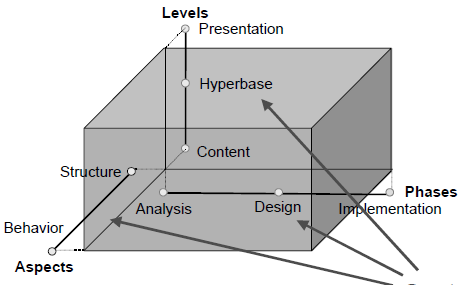
\includegraphics[width=5 in,totalheight=3 in]
{Ch1/Figuras/ScopeCustomisation.png}
 % UWAFramework2.png: 828x510 pixel, 96dpi, 21.90x13.49 cm, bb=0 0 621 382
\caption{Dise\~no conceptual del Framework UWA}\label{uwaFramework}
\end{center}
\end{figure}


\begin{figure}[t]
\begin{center}
 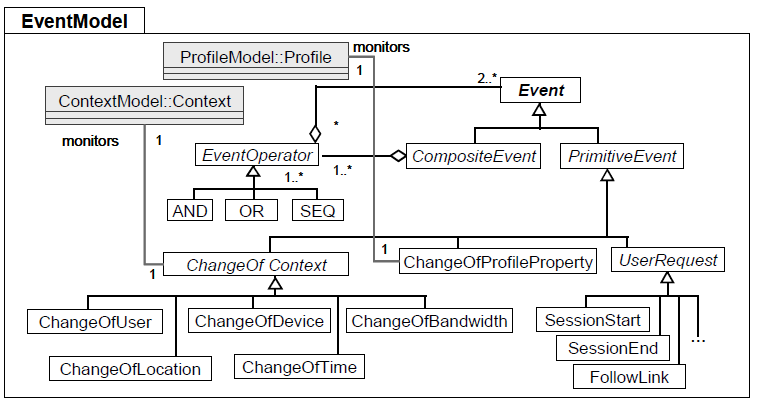
\includegraphics[width=4 in,totalheight=3 in]
{Ch1/Figuras/UWAEventModel.png}
 % UWAFramework2.png: 828x510 pixel, 96dpi, 21.90x13.49 cm, bb=0 0 621 382
\caption{Dise\~no conceptual del Fram}\label{uwaFramework}
\end{center}
\end{figure}



\section{Desde la perspectiva de la Ingeniería de Software}
%...
%(escribir todo esto como teoría de requerimientos).
%...
 
En este capítulo se han explicitado los fundamentos y desarrollos básicos de la evolución
de las aplicaciones sensibles al contexto. Introducimos la necesidad de que los mismos tuvieran un nivel dinámico sustentado en la teoría de coordinación de
contratos, ya que las definiciones más tradicionales no son suficientes para satisfacer los requerimientos del DHD.

En los capítulos siguientes, se abordará lo inherente a los contratos como pieza de software en base a la arquitectura, el diseño y la implementación en el campo de la Ingeniería de Software para describir las problemáticas, motivaciones,
el tipo de solución propuesta y un marco de conceptualización-definición (capítulos: \ref{cap:Introduccion} y \ref{cap:dhd} ) en un contexto de alta complejidad como lo ya expuesto, para tratar requerimientos funcionales derivados del mismo. 

Se tomarán en cuenta todas las convenciones realizadas sobre el DHD, haciendo foco en adelante sobre lo específicamente tecnológico, estableciéndose la intersección interdisciplinar entre las competencias de los usuarios expertos y los ingenieros de software como destinatarios principales de este trabajo de tesis doctoral. 

Es importante para el desarrollo de los próximos capítulos tener presente los siguientes interrogantes que se constituyen en el sentido sustentador para el uso de la teoría de Sistemas Colaborativos Sensibles al Contexto en las aplicaciones que integran al DHD. 


\begin{center}

\begin{tabular}[t]{|l|}
\hline
\rowcolor{gray}
Preguntas
\hline

%\beging{itemize}

\item ¿Cuáles son las variables que definen el contexto del usuario que\\
pueden ser usadas para recuperar información relevante? \\
\hline
\item ¿De qué forma puede modelarse el contexto del usuario? \\
\hline
\item ¿Cómo debe incorporarse el contexto a la búsqueda del usuario?\\
\hline
\item ¿Cómo deben presentarse los resultados derivados del contexto del
usuario?\\
\hline
\item ¿Cuál es la relación costo/beneficio de utilizar el contexto en la
recuperación de información?\\
\hline
\item ¿De qué forma se puede medir la relevancia de los resultados derivados del
contexto?\\
\hline
\item ¿En qué tipo de aplicaciones puede ser útil incorporar mecanismos
que\\
hagan uso del contexto para que logren robustez entregando información
relevante?\\
\hline
%\end{itemize}


\end{tabular}
\end{center}




\section{Conclusiones}

Este capítulo conforma una bisagra entre el universo real del DHD y
las limitaciones de su interpretación computacional. En este sentido, se ha focalizado en determinar cuáles son las fuentes concretas de la
materia prima (el ContextoDHD, sección \ref{sec:contextodhd}) para poder
producir soluciones (el Modelo Evolutivo, sección \ref{sec:sca})
a determinados efectos funcionales del DHD. De la misma manera inicia un
recorrido sobre el estado del arte de propuestas referentes en las que se basa
esta tesis. Entonces, desde este punto se mantendrán nuevas premisas aportadas
que permitirán especializar teorías y conceptos con una nueva entidad
apropiada para el DHD.

